\documentclass[portrait,final,paperwidth=92cm, paperheight=152cm,  fontscale=0.277]{baposter}
%a0paper,
\usepackage{calc}
\usepackage{graphicx}
\usepackage{amsmath}
\usepackage{amssymb}
\usepackage{relsize}
\usepackage{multirow}
\usepackage{rotating}
\usepackage{bm}
\usepackage{url}
\usepackage{setspace}
\usepackage{graphicx}
\usepackage{multicol}
\usepackage{siunitx}
\usepackage{vwcol} 
\usepackage{varwidth}
\usepackage{tikz}
\usepackage{graphicx}
\graphicspath{{/home/nicole/Documents/presentations/ipac2018/logos}{/home/nicole/Documents/presentations/ipac2018/tba-ipac18}}
\usetikzlibrary{calc}
%\usepackage{times}
%\usepackage{helvet}
%\usepackage{bookman}
\usepackage{palatino}
\newcommand\Tstrut{\rule{0pt}{2.6ex}}         % = `top' strut

\newcommand{\captionfont}{\footnotesize}

\graphicspath{{images/}{../images/}}
\usepackage{tikz}
\usetikzlibrary{shapes.misc}
\usetikzlibrary{shapes,arrows,decorations.markings,shadows,positioning}
\usetikzlibrary{snakes,backgrounds,spy}
\usepackage{tcolorbox}
\newcommand{\SET}[1]  {\ensuremath{\mathcal{#1}}}
\newcommand{\MAT}[1]  {\ensuremath{\boldsymbol{#1}}}
\newcommand{\VEC}[1]  {\ensuremath{\boldsymbol{#1}}}
\newcommand{\Video}{\SET{V}}
\newcommand{\video}{\VEC{f}}
\newcommand{\track}{x}
\newcommand{\Track}{\SET T}
\newcommand{\LMs}{\SET L}
\newcommand{\lm}{l}
\newcommand{\PosE}{\SET P}
\newcommand{\posE}{\VEC p}
\newcommand{\negE}{\VEC n}
\newcommand{\NegE}{\SET N}
\newcommand{\Occluded}{\SET O}
\newcommand{\occluded}{o}
\renewcommand{\baselinestretch}{-1.5} 
%%%%%%%%%%%%%%%%%%%%%%%%%%%%%%%%%%%%%%%%%%%%%%%%%%%%%%%%%%%%%%%%%%%%%%%%%%%%%%%%
%%%% Some math symbols used in the text
%%%%%%%%%%%%%%%%%%%%%%%%%%%%%%%%%%%%%%%%%%%%%%%%%%%%%%%%%%%%%%%%%%%%%%%%%%%%%%%%

%%%%%%%%%%%%%%%%%%%%%%%%%%%%%%%%%%%%%%%%%%%%%%%%%%%%%%%%%%%%%%%%%%%%%%%%%%%%%%%%
% Multicol Settings
%%%%%%%%%%%%%%%%%%%%%%%%%%%%%%%%%%%%%%%%%%%%%%%%%%%%%%%%%%%%%%%%%%%%%%%%%%%%%%%%
\setlength{\columnsep}{1.5em}
\setlength{\columnseprule}{0mm}

%%%%%%%%%%%%%%%%%%%%%%%%%%%%%%%%%%%%%%%%%%%%%%%%%%%%%%%%%%%%%%%%%%%%%%%%%%%%%%%%
% Save space in lists. Use this after the opening of the list
%%%%%%%%%%%%%%%%%%%%%%%%%%%%%%%%%%%%%%%%%%%%%%%%%%%%%%%%%%%%%%%%%%%%%%%%%%%%%%%%
\newcommand{\compresslist}{%
	\setlength{\itemsep}{1pt}%
	\setlength{\parskip}{0pt}%
	\setlength{\parsep}{0pt}%
}

%%%%%%%%%%%%%%%%%%%%%%%%%%%%%%%%%%%%%%%%%%%%%%%%%%%%%%%%%%%%%%%%%%%%%%%%%%%%%%
%%% Begin of Document
%%%%%%%%%%%%%%%%%%%%%%%%%%%%%%%%%%%%%%%%%%%%%%%%%%%%%%%%%%%%%%%%%%%%%%%%%%%%%%
\begin{document}

%%%%%%%%%%%%%%%%%%%%%%%%%%%%%%%%%%%%%%%%%%%%%%%%%%%%%%%%%%%%%%%%%%%%%%%%%%%%%%
%%% Here starts the poster
%%%---------------------------------------------------------------------------
%%% Format it to your taste with the options
%%%%%%%%%%%%%%%%%%%%%%%%%%%%%%%%%%%%%%%%%%%%%%%%%%%%%%%%%%%%%%%%%%%%%%%%%%%%%%
\definecolor{silver}{cmyk}{0,0,0,0.3}
\definecolor{black}{cmyk}{0,0,0.0,1.0}
\definecolor{darkYellow}{cmyk}{0,0,1.0,0.5}
\definecolor{darkSilver}{cmyk}{0,0,0,0.1}

\definecolor{KTHBlue}{cmyk}{.71,.37,0.07,0}
\definecolor{KTHsilver}{cmyk}{0,0,0,0.35}
\definecolor{KTHbeige}{cmyk}{0,0.03,0.19,0.04}


\begin{poster}{
  % Poster Options
	% Show grid to help with alignment
	grid=false,
	columns=6,
	% Column spacing
	colspacing=1em,
	% Color style
	bgColorOne=white,
	bgColorTwo=white,
	borderColor=KTHBlue,
	headerColorOne=black,
	headerColorTwo=KTHBlue,
	headerFontColor=white,
	boxColorOne=white,
	boxColorTwo=KTHBlue,
	% Format of textbox
	textborder=roundedleft,
	% Format of text header
	eyecatcher=true,
	headerborder=closed,
	headerheight=0.085\textheight,
	%  textfont=\sc, An example of changing the text font
	headershape=roundedright,
	headershade=shadelr,
	headerfont=\Large\bf\textsc, %Sans Serif
	textfont={\setlength{\parindent}{0em}},
	boxshade=plain,
	%  background=shade-tb,
	background=plain,
	linewidth=2pt
}
% Eye Catcher
{
	
	%\makebox[3em][l]{
		
} %}
% Title
{\bf\textsc{Photoinjector Optimization \\ Studies at the AWA}}%\vspace{10em}}
% Authors
{\vspace{1em}
	N. Neveu\textsuperscript{1}, L. Spentzouris, Illinois Institute of Technology, Chicago, IL, USA \\
	J. Larson, J. G. Power, \textsuperscript{1}Argonne National  Laboratory, Lemont, IL, USA \\
    }
% University logo
{% The makebox allows the title to flow into the logo, this is a hack because of the L shaped logo.
	%\makebox[3em][r]{
		\includegraphics[height=9em]{logos/combo_logo}%}
}




%%%%%%%%%%%%%%%%%%%%%%%%%%%%%%%%%%%%%%%%%%%%%%%%%%%%%%%%%%%%%%%%%%%%%%%%%%%%%%
\headerbox{AWA Facility}{name=problem,column=0,row=0, span=2}{
%%%%%%%%%%%%%%%%%%%%%%%%%%%%%%%%%%%%%%%%%%%%%%%%%%%%%%%%%%%%%%%%%%%%%%%%%%%%%%
The Argonne Wakefield Accelerator (AWA) Facility houses two rf photoinjectors.
Simulation codes used for experiments at the AWA include: PARMELA, GPT, 
ASTRA, and more recently OPAL. 
The latter is the code used for all simulations in this 
study. 
We also take advantage of the computing resources provided
by the LCRC at ANL. Access to the 
Blues, and recently installed Bebop clusters has significantly
increased simulation productivity by providing the capability to run 
all simulations in parallel, and large optimization cases
on many cores.
}

%%%%%%%%%%%%%%%%%%%%%%%%%%%%%%%%%%%%%%%%%%%%%%%%%%%%%%%%%%%%%%%%%%%%%%%%%%%%%%
\headerbox{Beam Line Layout}{name=beamline,column=2,row=0,span=4, bottomaligned=problem}{
%%%%%%%%%%%%%%%%%%%%%%%%%%%%%%%%%%%%%%%%%%%%%%%%%%%%%%%%%%%%%%%%%%%%%%%%%%%%%%
\centering
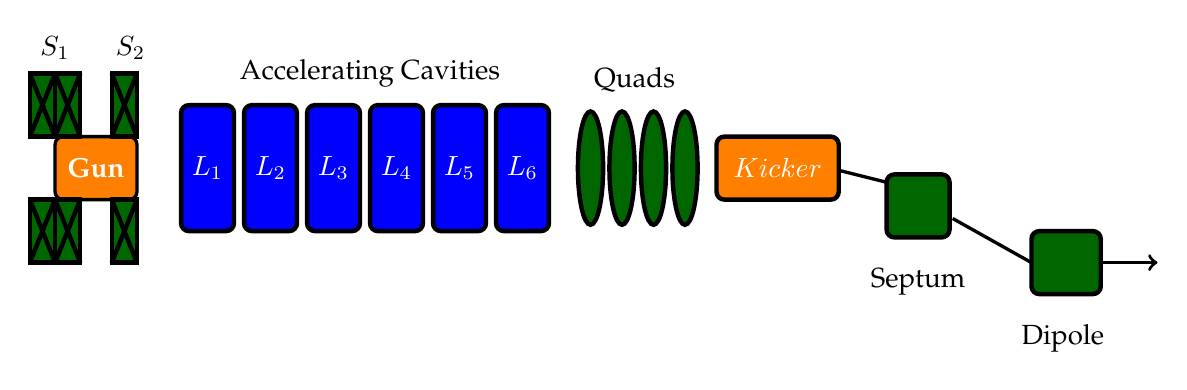
\begin{tikzpicture}[scale=0.8, text=black]
\def \gunleft {-1.0}
\def \gunright {0.3}
\def \loneright {1.0}
\def \ltworight {2.0}
\def \lthreeright {3.0}
\def \lfourright {4.0}
\def \lfiveright {5.0}
\def \lsixright {6.0}
\def \quadone {7.5}
\def \quadfour{16}

\draw[fill=orange, very thick, rounded corners =0.1cm] (\gunleft,0.5)rectangle (\gunright,1.5) node[pos=.5, white] {\textbf{Gun}} ;

%S1
\node[] at (-1,2.9) {$S_1$};
\draw[ultra thick, fill=black!60!green] (-1.4,-0.5)rectangle  (-1.0,0.5) node[pos=.5, white] {} ;
\draw[black, ultra thick] (-1.4,-0.5) -- (-1.0,0.5);
\draw[black, ultra thick] (-1.4,0.5) -- (-1.0,-0.5);
\draw[ultra thick, fill=black!60!green] (-1.4,1.5)rectangle  (-1.0,2.5) node[pos=.5, white] {} ;
\draw[black, ultra thick] (-1.4,1.5) -- (-1.0,2.5);
\draw[black, ultra thick] (-1.4,2.5) -- (-1.0,1.5);
%S2

\draw[ultra thick, fill=black!60!green] (-1.0,-0.5)rectangle  (-0.6,0.5) node[pos=.5, white] {} ;
\draw[black, ultra thick] (-1.0,-0.5) -- (-0.6,0.5);
\draw[black, ultra thick] (-1.0,0.5) -- (-0.6,-0.5);
\draw[ultra thick, fill=black!60!green] (-1.0,1.5)rectangle  (-0.6,2.5) node[pos=.5, white] {} ;
\draw[black, ultra thick] (-1.0,1.5) -- (-0.6,2.5);
\draw[black, ultra thick] (-1.0,2.5) -- (-0.6,1.5);

%S3
\node[] at (0.2,2.9) {$S_2$};
\draw[ultra thick, fill=black!60!green] (-0.1,-0.5) rectangle  (0.3,0.5) node[pos=.5, white] {};
\draw[black, ultra thick] (-0.1,-0.5) -- (0.3,0.5);
\draw[black, ultra thick] (-0.1,0.5) -- (0.3,-0.5);
\draw[ultra thick, fill=black!60!green] (-0.1,1.5) rectangle  (0.3,2.5) node[pos=.5, white] {};
\draw[black, ultra thick] (-0.1,1.5) -- (0.3,2.5);
\draw[black, ultra thick] (-0.1,2.5) -- (0.3,1.5);
%Linac drawings 
\node[] at (4,2.5) {Accelerating Cavities};
\draw[fill=blue, ultra thick, rounded corners =0.1cm] (\loneright,0)rectangle  ({\loneright+0.84},2) node[pos=.5, white] {$L_1$} ;
\draw[fill=blue, ultra thick, rounded corners =0.1cm] (\ltworight,0)rectangle  ({\ltworight+0.84},2) node[pos=.5, white] {$L_2$};
\draw[fill=blue, ultra thick, rounded corners =0.1cm] (\lthreeright,0)rectangle ({\lthreeright+0.84},2) node[pos=.5, white] {$L_3$};
\draw[fill=blue, ultra thick, rounded corners =0.1cm] (\lfourright,0)rectangle ({\lfourright+0.84},2) node[pos=.5, white] {$L_4$};
\draw[fill=blue, ultra thick, rounded corners =0.1cm] (\lfiveright,0)rectangle ({\lfiveright+0.84},2) node[pos=.5, white] {$L_5$};
\draw[fill=blue, ultra thick, rounded corners =0.1cm] (\lsixright,0)rectangle ({\lsixright+0.84},2) node[pos=.5, white] {$L_6$};

%current optimization point
%\node[draw, fill=yellow, star, star points=5, star point ratio=0.6, minimum size=0.1cm]
%at (12.5,1.0) {$z_1$};


%Quad drawings
\node[] at (8.2,2.4) {Quads};
\draw[fill=black!60!green, ultra thick] (\quadone, 1.0) ellipse (0.2cm and 0.9cm);
\draw[fill=black!60!green, ultra thick] (\quadone+0.5, 1.0) ellipse (0.2cm and 0.9cm);
\draw[fill=black!60!green, ultra thick] (\quadone+1.0, 1.0) ellipse (0.2cm and 0.9cm);
\draw[fill=black!60!green, ultra thick] (\quadone+1.5, 1.0) ellipse (0.2cm and 0.9cm);

%Line between kicker and septum
\draw[very thick] (\lsixright+5.3,1.0) -- (12.5,0.7);

%Kicker 
\draw[fill=orange, ultra thick, rounded corners =0.1cm] (\lsixright+3.5,0.5)rectangle ({\lsixright+0.84+4.6},1.5) node[pos=.5, white] {$Kicker$};

%Septum
\node[] at (12.7,-0.8) {Septum};
\draw[fill=black!60!green, ultra thick, rounded corners =0.1cm] (12.2,0.9)rectangle ({13.2},-0.1) node[pos=.5, white] {};
%\draw[latex-latex] (\gunleft,-5.0) -- (14,-5.0) ;
%\foreach \x in  {0.3, 1.0, 3.5, 5.0, 7.0, 8.5, 10, 12.5} %tick marks
%\draw[shift={(\x,-5.0)},color=black] (0pt,3pt) -- (0pt,-3pt);
%\foreach \x in {0.3, 1.0, 3.5, 5.0, 7.0, 8.5, 10, 12.5}
%\draw[shift={(\x,-5.2)},color=black] (0pt,0pt) node[below] {$\x$};

%Line between kicker and septum
\draw[very thick] (13.25,0.2) -- (14.5,-0.5);

%Dipole
\node[] at (15,-1.7) {Dipole};
\draw[fill=black!60!green, ultra thick, rounded corners =0.1cm] (14.5,0.0)rectangle ({15.6},-1.0) node[pos=.5, white] {};

%Line between septum and dipole
\draw[very thick, ->] (15.6,-0.5) -- (16.5,-0.5);
%Second set of quads

%Straight through
\draw[very thick] (15.6,-0.5) -- (16.5,-0.5);



\end{tikzpicture}	

Partial beam line layout at the AWA.

}



%%%%%%%%%%%%%%%%%%%%%%%%%%%%%%%%%%%%%%%%%%%%%%%%%%%%%%%%%%%%%%%%%%%%%%%%%%%%%%
\headerbox{Model Based Method: BOBYQA}{name=bob,column=0,below=problem, span=6}{%, bottomaligned=conclusion}{
%%%%%%%%%%%%%%%%%%%%%%%%%%%%%%%%%%%%%%%%%%%%%%%%%%%%%%%%%%%%%%%%%%%%%%%%%%%%%%
\noindent
Last year, we began with the optimization of 
the high charge (\SI{40}{nC}) photoinjector at the AWA. 
The simulation model included the gun, two solenoids, 
and six accelerating cavities.
We choose ten variables for the optimization parameters: 
laser radius, laser full width half maximum, solenoid strength ($S_2$), 
gun cavity phase, and the six accelerating cavity phases ($\phi_{L_1}-\phi_{L_6}$).

The objectives were emittance, and bunch length at the entrance of the quads. 
We choose to use a local optimization method that is 
freely available in the NLOPT package. 
Bounded Optimization By Quadratic Approximation (BOBYA), 
is a model based and derivative-free method 
that builds a quadratic using the results of simulation evaluations. 
The next point to evaluate is chosen by minimizing the quadratic.
The initial probe of the parameter space was done with 1,000 random simulations.
Simulations with the best emittance and bunch length were chosen 
as starting points for ten BOBYQA runs.
These local optimization runs were carried out until they converged.
The results from all ten runs were used to form a Pareto front
comparing transverse emittance and bunch length. 
Details of this work were presented at IPAC'17.
\vspace{-1em}

\begin{center}
	\begin{minipage}{0.5\textwidth}
The initial results were promising, and attempts to measure
several points on the Pareto front took place.
Experimentally, some of the parameter values were found to 
be outside the normal operating conditions at the AWA.
Using this experience, a second round of optimization 
was done using the same procedure and method. The boundaries for the second
round of optimization work can be found in the table below.
Note that $\phi_L=[\phi_{L_1},\ldots,\phi_{L_6}]$.

Several key points were learned from this work:
\begin{itemize}
	\item Varying the laser radius is unnecessary. 
	All points on the Pareto front	had a laser radius of \SI{9}{mm}, the maximum value (results of strong space charge).
	\item Phase boundaries were too large for gun and linac.
	\item Phase can be used for velocity bunching	
\end{itemize}
		
\vspace{3em}
		\begin{singlespace}
			\centering
			
			Parameter Bounds for Linac Optimization
			
			\begin{tabular}{ l *{3}{c}}
				\hline%\toprule
				\textbf{Variable} & \textbf{Range} & \textbf{Unit} \\
				\hline%\midrule
				Solenoid Strength & $ 50 \le S_2 \le 440$  & amps \\
				Phase of Gun & $-45 \le \phi_g \le 45$  & degrees \\
				Laser Radius  & $3.5 \le R \le 9$  & mm \\
				Laser FWHM & $1.5 \le T \le $10  & ps \\
				Cavity Phase & $-40 \le \phi_L \le 40$  & degrees \\
				\hline%\bottomrule	
			\end{tabular}
		\end{singlespace}
	\end{minipage}\hspace{1em}
	\begin{minipage}{0.48\textwidth}
		\centering
		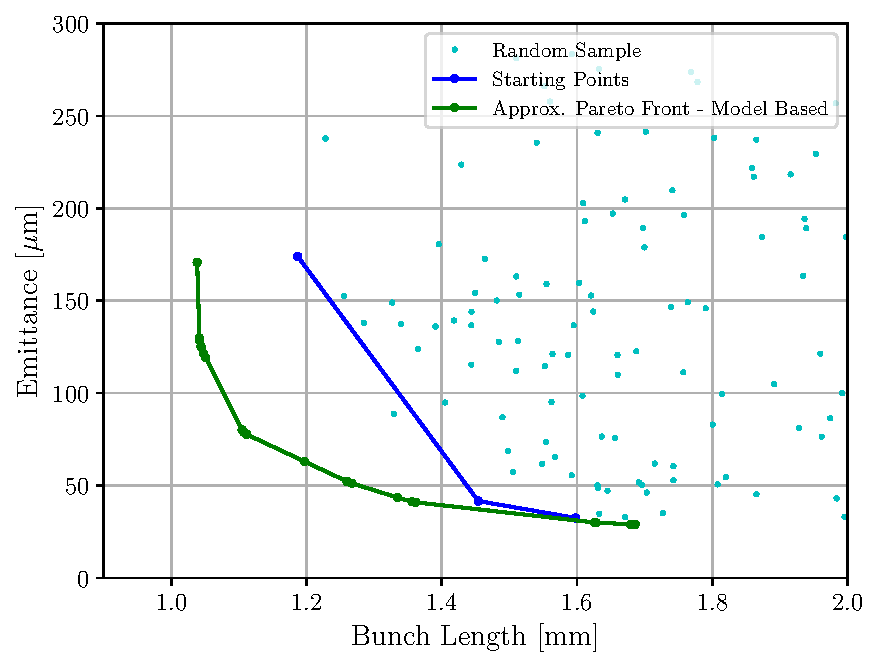
\includegraphics[width=1\textwidth]{THPMF049f2}
		
		Pareto front for adjusted variable bounds at \SI{40}{nC}. 
	\end{minipage}
	
\end{center}
}


%%%%%%%%%%%%%%%%%%%%%%%%%%%%%%%%%%%%%%%%%%%%%%%%%%%%%%%%%%%%%%%%%%%%%%%%%%%%%%
\headerbox{Genetic Algorithm}{name=kicker,column=0,row=0,span=6, below=bob}{
%%%%%%%%%%%%%%%%%%%%%%%%%%%%%%%%%%%%%%%%%%%%%%%%%%%%%%%%%%%%%%%%%%%%%%%%%%%%%%


\vspace{-2em}
\begin{center}
	\begin{minipage}{0.3\textwidth}
		\begin{singlespace}
				\begin{tabular}{ l *{2}{c}}
				\hline%\toprule
				\textbf{Variable} & \textbf{Range} \\
				\hline%\midrule
				Solenoid Strength & $ 350 \le S_1[A] \le 500$   \\
				Solenoid Strength & $ 170 \le S_2[A] \le 260$   \\
				Phase of Gun & $-30 \le \phi_g \le 0.0$  \\
				Laser FWHM & $1.5 \le T[ps] \le $10   \\
				Quadrupoles & $-8 \le K[Tesla] \le 8$  \\
				\hline%\bottomrule	
			\end{tabular}
		\end{singlespace}
	\end{minipage}	\hspace{20mm}
	\begin{minipage}{0.5\textwidth}
		\includegraphics[width=1\textwidth]{paper-pareto-ex-vs-rmss}
	\end{minipage}
\end{center}

}


%%%%%%%%%%%%%%%%%%%%%%%%%%%%%%%%%%%%%%%%%%%%%%%%%%%%%%%%%%%%%%%%%%%%%%%%%%%%%%
\headerbox{Conclusion}{name=ref,column=2,above=bottom, span=2}{%
%%%%%%%%%%%%%%%%%%%%%%%%%%%%%%%%%%%%%%%%%%%%%%%%%%%%%%%%%%%%%%%%%%%%%%%%%%%%%%
\noindent 


}

%%%%%%%%%%%%%%%%%%%%%%%%%%%%%%%%%%%%%%%%%%%%%%%%%%%%%%%%%%%%%%%%%%%%%%%%%%%%%%
\headerbox{Acknowlegements}{name=ref,column=4,above=bottom, span=2, above=bottom}{%
%%%%%%%%%%%%%%%%%%%%%%%%%%%%%%%%%%%%%%%%%%%%%%%%%%%%%%%%%%%%%%%%%%%%%%%%%%%%%%
\noindent 
We gratefully acknowledge the computing resources
provided on Bebop, a HPC cluster operated by the LCRC at ANL.
This work is supported by the U.S. DOE, OS,  
contract DE-AC02-06CH11357 and grant DE-SC0015479. 
Travel to IPAC'18 supported by the United States National Science Foundation, 
the Division of Physics of Beams of the American Physical Society, and TRIUMF.
\vspace{-1em}
\hfill
\begin{center}
	\includegraphics[width=0.1\textwidth]{logos/nsf}\hspace{1em}
\includegraphics[width=0.3\textwidth]{logos/DOE_logo_color_cmyk}\hspace{1em}
\includegraphics[width=0.1\textwidth]{logos/aps-logo}
\end{center}
}


\end{poster}%
%
\end{document}
